\subsection{Nhất quán dữ liệu giữa blockchain và MongoDB}

Mỗi thao tác nghiệp vụ quan trọng của hệ thống đều phải ghi đồng thời lên hai hệ lưu trữ tách biệt: sổ cái Hyperledger Fabric và cơ sở dữ liệu MongoDB. Hai lần ghi này không thể bọc chung trong một giao dịch nguyên tử (\textit{atomic}). Nếu ghi chuỗi khối trước rồi ghi cơ sở dữ liệu sau (\textit{chain-first}), một lỗi xảy ra ở bước ghi cơ sở dữ liệu — \textbf{sau khi} chuỗi khối đã ghi nhận thành công — sẽ làm hai bên lệch nhau; và vì sổ cái là bất biến nên không thể hoàn tác. Bảng~\ref{tab:dual-write} liệt kê ba điểm ghi kép cùng hậu quả khi lệch theo hướng \textit{chain-first}.

\begin{table}[H]
\centering
\caption{Ba điểm ghi kép và hậu quả khi lệch dữ liệu theo hướng chain-first}
\label{tab:dual-write}
\begin{tabularx}{\textwidth}{|L{0.32}|L{0.68}|}
\hline
\textbf{Thao tác} & \textbf{Hậu quả khi chuỗi khối thành công nhưng cơ sở dữ liệu lỗi} \\
\hline
\pkg{SubmitVote} & Chuỗi khối có phiếu, cơ sở dữ liệu thiếu $\rightarrow$ số phiếu hai bên lệch $\rightarrow$ lệnh \pkg{CommitMerkleRoot} bị từ chối khi đóng cuộc bầu cử. \\
\hline
\pkg{CommitMerkleRoot} & Chuỗi khối đã đóng, cơ sở dữ liệu còn \pkg{ACTIVE} $\rightarrow$ thử lại bị từ chối (do tính idempotent) $\rightarrow$ cuộc bầu cử bị kẹt. \\
\hline
\pkg{RevealVoteCompact} & Chuỗi khối đã dùng \pkg{revealKey}, cơ sở dữ liệu thiếu $\rightarrow$ cử tri thử lại bị báo ``revealKey đã dùng'' $\rightarrow$ không thể tiết lộ lại. \\
\hline
\end{tabularx}
\end{table}

\subsubsection{Giải pháp 1 --- Ghi cơ sở dữ liệu trước kèm trạng thái trung gian}

Hai thao tác \pkg{SubmitVote} và đóng cuộc bầu cử áp dụng mô hình \textit{Write-DB-First}: ghi cơ sở dữ liệu ở một trạng thái trung gian \textbf{trước}, rồi mới gọi chuỗi khối, sau đó xác nhận lại cơ sở dữ liệu. Trình tự gồm bốn bước:

\begin{itemize}
    \item \textbf{Bước 1 --- Ghi trạng thái trung gian:} ghi bản ghi với trạng thái \pkg{Vote.status = PENDING\_CHAIN} (đối với phiếu) hoặc \pkg{Election.status = CLOSING} (đối với đóng cuộc bầu cử), trường \pkg{blockchainRef} để trống. Vì cơ sở dữ liệu được ghi trước, ràng buộc duy nhất \pkg{(electionId, voterId)} chặn bỏ phiếu trùng ngay tại bước này — trước cả khi chạm tới chuỗi khối; riêng \pkg{CLOSING} còn đóng vai trò khóa chống đóng cuộc bầu cử đồng thời.

    \item \textbf{Bước 2 --- Gọi chuỗi khối:} thực thi giao dịch \textit{invoke} tương ứng.

    \item \textbf{Bước 3 --- Chuỗi khối thành công:} xác nhận cơ sở dữ liệu, chuyển trạng thái sang \pkg{CONFIRMED} (hoặc \pkg{CLOSED}) và ghi \pkg{blockchainRef} bằng mã giao dịch trả về.

    \item \textbf{Bước 4 --- Chuỗi khối báo lỗi:} truy vấn lại chuỗi khối (\pkg{GetVote} hoặc \pkg{GetMerkleRoot}) để phân định, vì chuỗi khối là \textbf{nguồn sự thật}: nếu dữ liệu \textit{đã} có trên chuỗi khối thì xác nhận cơ sở dữ liệu và phục hồi mã giao dịch từ kết quả truy vấn; nếu \textit{chưa} có thì hoàn tác cơ sở dữ liệu (xóa phiếu \pkg{PENDING\_CHAIN} hoặc đưa cuộc bầu cử về \pkg{ACTIVE}) rồi ném lỗi để người dùng thử lại.
\end{itemize}

Hình~\ref{fig:submit-vote-write-db-first} trình bày hiện thực của mô hình này trong thao tác nộp phiếu.

\begin{figure}[H]
    \centering
    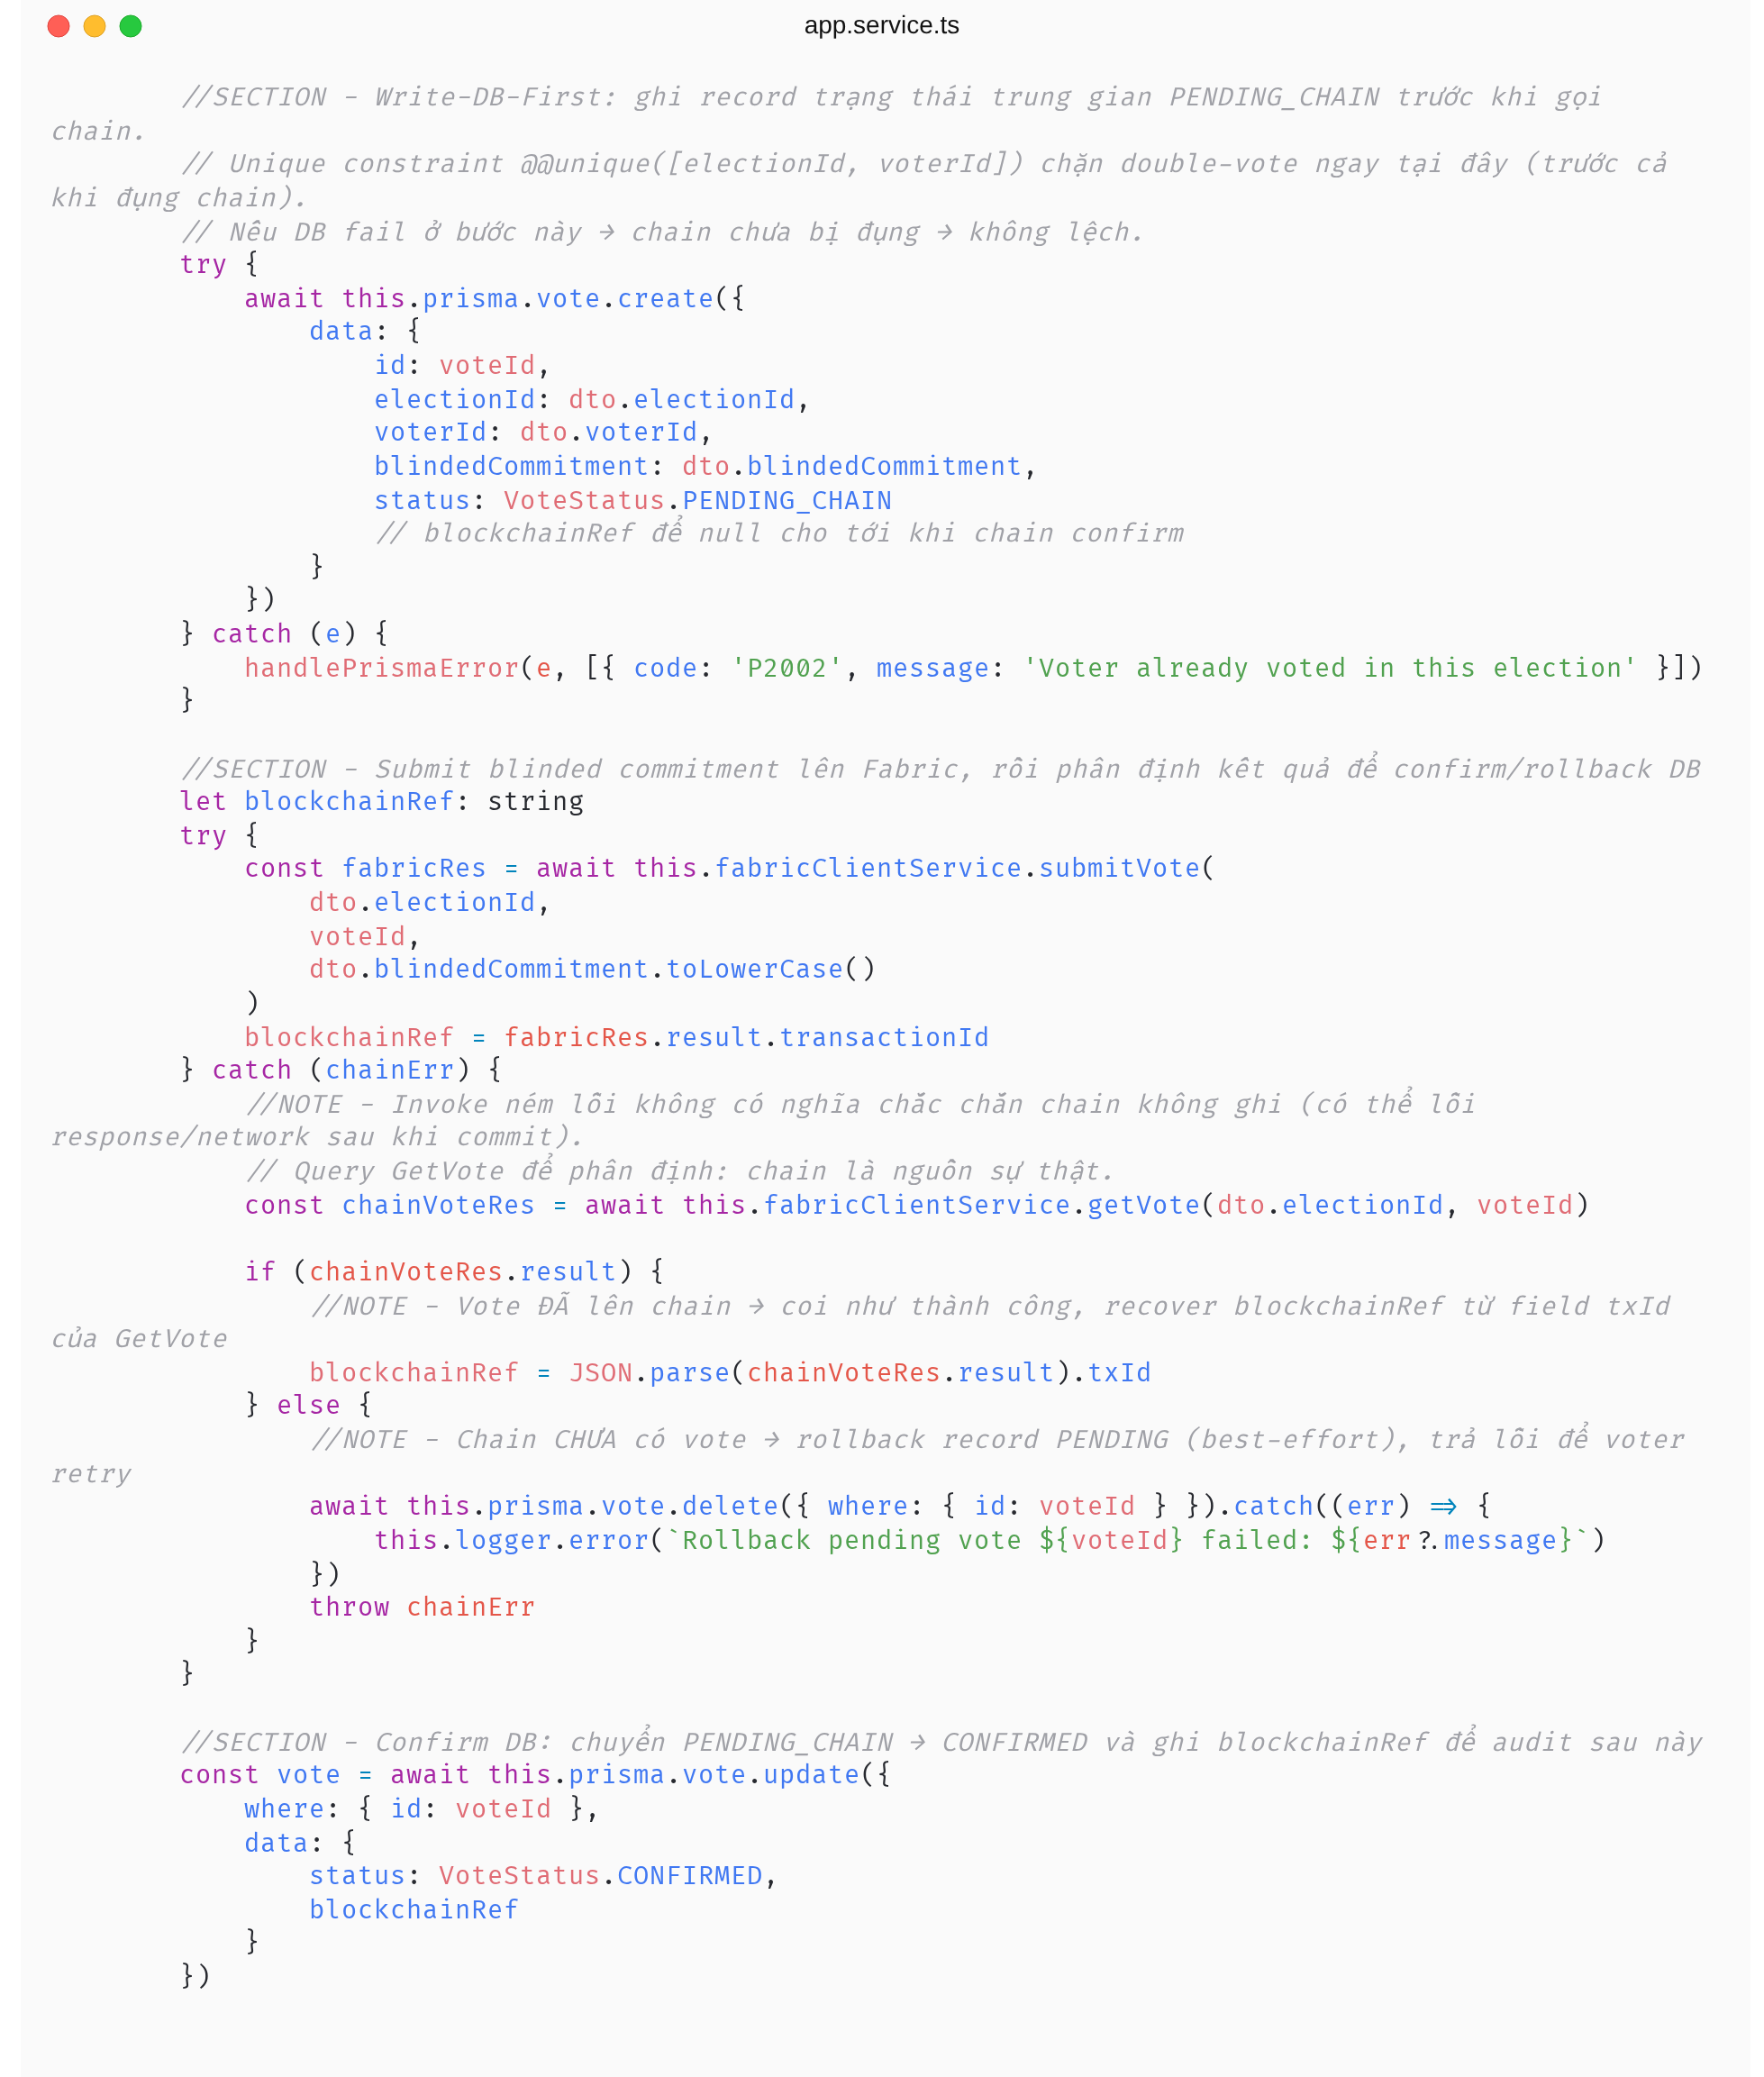
\includegraphics[width=\textwidth, keepaspectratio]{Figures/code/submit-vote-write-db-first.png}
    \caption{Mô hình Write-DB-First trong thao tác nộp phiếu \pkg{submitBlindedCommitment}}
    \label{fig:submit-vote-write-db-first}
\end{figure}

\subsubsection{Giải pháp 2 --- Giữ chain-first kèm tự phục hồi khi thử lại}

Thao tác \pkg{RevealVoteCompact} không đổi thứ tự ghi (vẫn chuỗi khối trước, cơ sở dữ liệu sau) vì \pkg{revealKey} là khóa idempotent tự nhiên trên chuỗi khối. Khi lệnh \textit{invoke} báo lỗi, hệ thống truy vấn \pkg{GetUsedReveal}: nếu chuỗi khối \textit{chưa} có \pkg{revealKey} thì đây là lỗi thật, ném tiếp; nếu chuỗi khối \textit{đã} có (và danh sách ứng viên khớp) thì coi là thử lại sau lỗi một phần, hệ thống ghi lại bản ghi cơ sở dữ liệu với \pkg{blockchainRef} để trống. Ràng buộc duy nhất \pkg{(electionId, revealKey)} vẫn ném lỗi nếu cơ sở dữ liệu đã có bản ghi, do đó tấn công phát lại thật vẫn bị chặn — chỉ phục hồi khi cơ sở dữ liệu còn trống.

\subsubsection{Tiến trình đồng bộ nền (Reconciler)}

Hai giải pháp trên xử lý lỗi trong luồng đồng bộ của yêu cầu. Trường hợp tiến trình \textit{sập} giữa bước gọi chuỗi khối và bước xác nhận sẽ để lại bản ghi kẹt ở trạng thái trung gian. Một tiến trình đồng bộ nền (\textit{reconciler}) chạy theo lịch \pkg{@Cron} của \pkg{@nestjs/schedule} đảm nhiệm việc dọn dẹp: định kỳ quét các bản ghi kẹt \textbf{cũ hơn} một ngưỡng thời gian (tránh tranh chấp với yêu cầu đang chạy), có cờ chống chồng lấn chu kỳ:

\begin{itemize}
    \item Phiếu còn \pkg{PENDING\_CHAIN}: truy vấn \pkg{GetVote} --- nếu có trên chuỗi khối thì chuyển \pkg{CONFIRMED}, nếu không thì xóa bản ghi.
    \item Cuộc bầu cử còn \pkg{CLOSING}: truy vấn \pkg{GetMerkleRoot} --- nếu đã cố định thì chuyển \pkg{CLOSED} và phục hồi mã giao dịch, nếu không thì giữ nguyên chờ quản trị viên thử lại.
\end{itemize}

\begin{figure}[H]
    \centering
    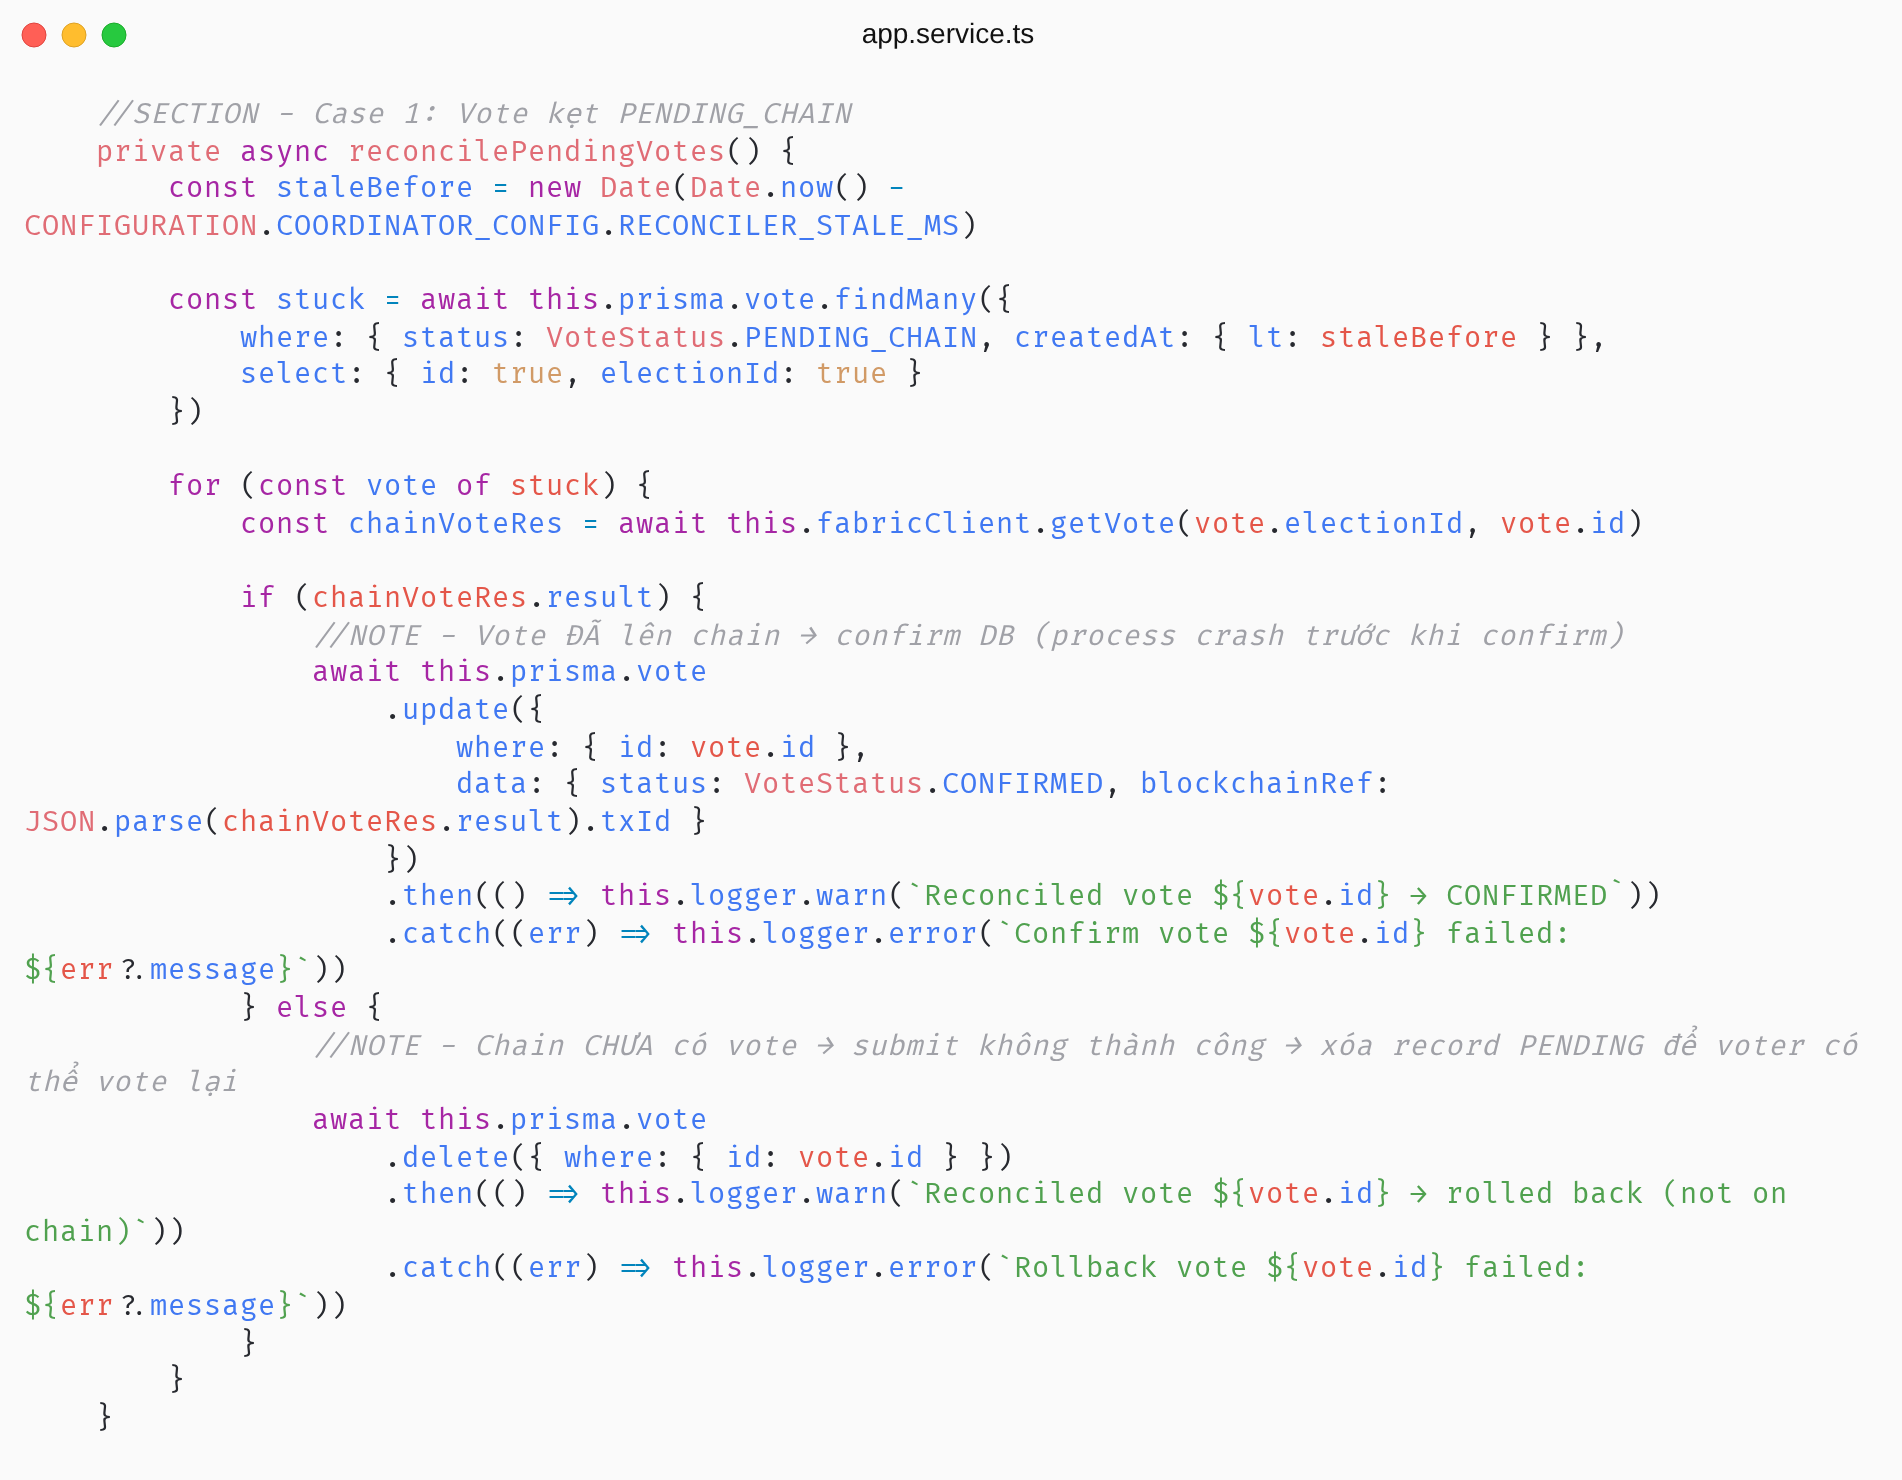
\includegraphics[width=\textwidth, keepaspectratio]{Figures/code/reconciler-pending-vote.png}
    \caption{Tiến trình đồng bộ nền đối chiếu phiếu \pkg{PENDING\_CHAIN} với chuỗi khối}
    \label{fig:reconciler-pending-vote}
\end{figure}

\subsubsection{Hệ quả về bất biến đọc dữ liệu}

Do chuỗi khối là nguồn sự thật, một phiếu chỉ được coi là hợp lệ khi đã \pkg{CONFIRMED}. Vì vậy mọi hàm đọc phiếu (đếm phiếu, dựng cây Merkle khi đóng, lọc danh sách phiếu) đều \textbf{mặc định lọc} \pkg{status = CONFIRMED} để khớp đúng tập phiếu thực sự có trên chuỗi khối. Hai ngoại lệ được giữ \textit{không phụ thuộc trạng thái} một cách có chủ đích: kiểm tra bỏ phiếu trùng khi khởi tạo phiên (phiếu \pkg{PENDING\_CHAIN} vẫn phải tính là ``đã bỏ phiếu'' để giữ chỗ) và thao tác xác minh phiếu phục vụ điều tra (cần thấy cả phiếu \pkg{PENDING\_CHAIN} để phát hiện lệch dữ liệu). Đây là mô hình \textit{nhất quán cuối} (\textit{eventual consistency}): trong khoảng chuỗi khối tạm thời không phản hồi, một phiếu có thể nằm ở \pkg{PENDING\_CHAIN} cho tới khi tiến trình đồng bộ nền đưa nó về trạng thái cuối cùng.
